\chapter[Information spreading]{Information spreading \raisebox{.3\baselineskip}{\normalsize\footnotemark}}
\footnotetext{Most of this chapter is taken from \href{https://github.com/Halolegend94/uni_social_behavioral_networks/blob/master/chapters/ch01-meme-flow.tex}{this repo} by \href{https://github.com/Halolegend94}{Cristian Di Pietrantonio}.}

On the web, information is published by one or more \emph{sources} and often spreads quickly to other parties. The most popular kind of information that spreads quickly is a meme. From \href{https://en.wikipedia.org/wiki/Meme}{Wikipedia}:

\begin{defn}[Meme]
	A meme is an idea, behavior, or style that spreads from person to person within a culture - often with the aim of conveying a particular phenomenon, theme or meaning represented by the meme.
\end{defn}

In this chapter we are going to define some mathematical models that describes the spread of information.\\
Let's note that in this case, unlike in the models seen in section [\ref{sec:users-behaviors}], the models work on the graph without changing it.

\section{Push}

First, a source node picks a neighbor \uar\ and sends to it the meme.

Then, each node that contains the meme choose a random neighbor and sends to it the meme, iteratively.


\section{Pull}

As in the previous model, the information starts in a single node.

Each node $x$ in the network, that doesn't contain the meme, chooses a neighbor $y$ \uar; if $y$ has the information, $x$ obtains the information too.

The procedure repeats many times, but the upper bound of the number of iterations is given by the number of rounds necessary to spread the ifnromation in the whole graph, that depends on the structure of the graph. For example, a star will require much less time than a chain.

This model can be useful to choose the best node to advertise a product.

\section{The Trace Spreading Model}

In this model for meme flow, nodes can receive or take information from other nodes, enabling the spread of the meme. They can also publish the same meme independently (without ``copying'' each other).

Whenever a node publishes information, a timestamp of the event is also available.

At the end, considering a particular meme, all we can see is a bunch of nodes having published with an associated timestamp. What we would like to know is the \emph{social graph} that links these nodes, i.e., who retrieves information from who. Clearly, we can't obtain a perfect reconstruction of the graph, but we can approximate it based on \textit{cascades} or \textit{traces} of the memes.

\begin{defn}[Trace]
    A trace is a sequence of nodes ordered by their timestamp.\\
    Usually we write it as ``\texttt{$v_1$ -> $v_1$ -> $v_2$ -> $t_2$ -> $\cdots$ -> $t_{n-2}$ -> $v_n$}'', where $v_i$ are nodes (or vertex of the social graph) and $t_i$ are times elapsed from $v_i$ to $v_{i+1}$.
\end{defn}

Define an undirected graph $G = (V, E)$, according to the Trace spreading model: \label{trace-spreading}
\begin{enumerate}
    \item Let $V$ be the set of nodes that holds the information of interest;
    \item Pick a single source of information, chosen \uar;
    \item $e = \{v, v'\} \in E$ iif information propagated from $v$ to $v'$, $v, v' \in V$ (the actual direction is not important, as you will notice later);
    \item Each edge $e = \{v, v'\}$ has a \emph{weight} $w(e)$ sampled \iid in $\emph{Exp}(\lambda)$, which represent the time needed for the information to propagate from $v$ to $v'$ (in fact, for our purpose, any \textbf{continuous} distribution will do);
    \item Build a trace following the shortest path tree from the source.
\end{enumerate}

From this model and the relative traces, we want to find an efficient algorithm that reconstructs the underlying graph with a certain confidence.

\begin{qst}
    How may traces do we need to reconstruct the graph?
\end{qst}

\section{The First-Edge Algorithm}
We can reconstruct (in most cases) the graph $G=(V, E)$ with high probability with a simple algorithm:
 
\begin{lstlisting}[caption={The first-edge algorithm},label={lst:first-edge}]
FirstEdge($\pi_1, \pi_2, \ldots, \pi_t$)   //the set of traces
	$E \gets \emptyset$   //the set of edges in the graph
	for $i = 1, \ldots, t$   //t = number of traces
		$E \gets E \cup \left\{\left( \pi_i(1), \pi_1(2) \right)\right\}$
\end{lstlisting}

Since the algorithm adds one edge for each trace, intuitively we would need as many traces as edges, to find all the edges.

What the algorithm does is simply adding an edge between the first and second node in a trace, for every trace. That is because we can only be sure about the existence of that edge: the first node in a trace is the source (for that trace), since it has the lowest timestamp, the second node, which has the second lowest timestamp, could only get the information from the first node.

\begin{ex}
    Let pick the execution of the trace spreading model [\ref{trace-spreading}] in [\ref{fig:first-edge-ex}] as an example: the node $A$, marked with a double line, is chosen as the source, then each edge is assigned a random weight, then the shortest path is followed and each node is labeled with the timestamp at which the meme reaches it. The resulting trace is \texttt{$\pi_1$ = \textbf{A -> C} -> B -> D}.
    \begin{figure}[h!]
        \centering
        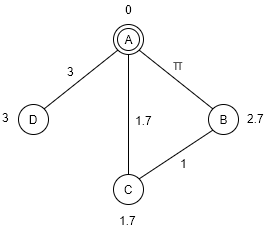
\includegraphics[scale=0.7]{first_edge_ex}
        \caption{First edge example}
        \label{fig:first-edge-ex}
    \end{figure}

    The following traces could be:\\
    \texttt{$\pi_2$ = \textbf{A -> B} -> D -> C},\\
    \texttt{$\pi_3$ = \textbf{C -> B} -> A -> D},\\
    \texttt{$\pi_1$ = \textbf{D -> A} -> B -> C},\\
    \texttt{$\pi_1$ = \textbf{A -> D} -> B -> C}.
\end{ex}

\begin{thm}[First Edge correctness]\label{thm:first-edge}
    Let $G=(V,E)$, $n=|V|$, $\Delta$ = max degree of $G=$, $t=$ number of traces. The output of the algorithm [\ref{lst:first-edge}] will be equal to $E(G)$, i.e., the algorithm will be correct, with probability $\geq 1 - \frac{1}{n^2}$ if $t \geq 2 n \Delta \ln(n)$.
\end{thm}

The high level meaning of the theorem is: the algorithm will give an exact answer if it is fed with enough traces.

Note that each trace is generated \iid with the trace spreading model in [\ref{trace-spreading}], by assigning new random weights and choosing a new random source.

\begin{lem}
    Let ${u,v} \in E(G)$, $n=|V|$; then, $\Pr{\text{a random trace } \pi \text{ begins with } u,v} = \frac{1}{n \deg(u)}$.
\end{lem}

\begin{proof}
    \begin{flalign*}
        &\Pr{\pi \text{ begins with } u,v} =&\\
        &=\Pr{\text{the random soursce is } u \text{, and } v \text{ is the first neighbor of } u \text{ to be informed}}&\\
        &= \Pr{\text{the soursce is } u} \cdot \Pr{\{u,v\} \text{ is the shortest edge incident on } u \text{ | source is } u}&\tag{by Bayes [\ref{eq-bayes}]}\\
        &= \frac{1}{n} \cdot \frac{1}{\deg u}&
    \end{flalign*}
    Note that, in the last step, $1/n$ is due to the fact that the source is chosen \uar, and $1/\deg(u)$ to the fact that each edge outgoing from $u$ has the same probability of being the shortest, since all the weights of these edges are taken from the same probability distribution (\textit{symmetry argument}), and the probability that two edges have the same weight is 0, since that distribution is continuous.
\end{proof}

\begin{lem}
    For any ${u,v} \in E(G)$, $\Pr{\text{a random trace } \pi \text{ begins with } u,v \text{ or } v,u} \geq \frac{2}{n \Delta}$.
\end{lem}

\begin{proof}
    \begin{flalign*}
    &\Pr{\pi \text{ begins with } u,v \text{ or } v,u}=&\\
    &= \Pr{\pi \text{ begins with } u,v} + \Pr{\pi \text{ begins with } v,u} - \Pr{\pi \text{ begins with } u,v \text{ \textbf{and} it begins with } v,u}&\tag{by [\ref{eq:prob-or}]}\\
    &= \Pr{\pi \text{ begins with } u,v} + \Pr{\pi \text{ begins with } v,u} &\tag{since the third probability is 0}\\
    &\frac{1}{\deg(u)} + \frac{1}{\deg(u)} \geq \frac{2}{n \Delta}&\tag{because $\Delta$ is greater or equal than any degree}
    \end{flalign*}
\end{proof}

Now our aim is to demonstrate that every ${u,v} \in E(G)$ appears at the beginning of a trace with positive probability, so that the expected value will be sufficiently high with enough traces.

\begin{lem}
    Let ${u,v} \in E(G)$, suppose we are given $t \geq 2n \Delta \ln(n)$ traces,\\
    $\Pr{\text{at least one trace begins with } u,v \text{ or } v,u} \geq 1 - \frac{1}{n^4}$.
\end{lem}

\begin{proof}
    Let $A_i$ be the event ``\textit{trace $i$ does not begin with $u,v$, nor it does begin with $v,u$}''.
    \begin{flalign*}
        &\Pr{A_1 \wedge A_2 \wedge \ldots \wedge A_t} = &\\
        &=\Pr{u,v \text{ or } v,u \text{  never appear at the beginning of a trace}}&\\
        &=\prod_{i=0}^{n}\Pr{E_i}&\tag{by [\ref{eq:prob}]}\\
        &\leq \left(1 - \frac{2}{n \Delta}\right)^t&\\
        &\leq \left(e^{-\frac{2}{n \Delta}}\right)^t&\tag{by [\ref{eq:e-x}]}\\
        &\leq \left(e^{-\frac{2}{n \Delta}}\right)^{2n \Delta \ln(n)}& \tag{because $2n \Delta \ln(n)$ is the smallest value that $t$ may assume}\\
        &=e^{-4 \ln(n)} = \frac{1}{n^4}&\tag{by [\ref{eq:log-prop}]}
    \end{flalign*}
    Therefore the lemma is demonstrated, since we proved that the probability of the complement of our claim is $1/n^4 = 1 - (1-1/n^4)$.
\end{proof}

\begin{proof}[Proof of Theorem \ref{thm:first-edge}]
    Let $B_{u,v}$ be the event ``\textit{no trace begins with $u,v$ or $v,u$}'' = ``\textit{the algorithm [\ref{lst:first-edge}] doesn't learn about the edge {$u,v$}}''.
    \begin{flalign*}
        &\Pr{\bigvee_{\{u,v\} \in E(G)} B_{\{u,v\}}}
        \leq \sum_{\{u,v\} \in E(G)} \Pr{B_{\{u,v\}}}
        \leq \sum_{\{u,v\} \in E(G)} n^{-4}
        \leq n^2 \cdot n^{-4} = n^{-2}&
    \end{flalign*}
    where $n^2$ is an upper bound of $|E(G)|$.\\
    The theorem is shown, since the complement of the bad event is what we were looking for.
\end{proof}
